\chapter{関連研究}
本研究では犬の一人称視点動画からの犬の活動分類を行う.人間のライフログとしての一人称動画の分類や,車載映像からの車の行動推定,第三者視点での動画分類,音声を用いた動画分類などについて紹介し,本研究との関連を述べる.

\section{タフ・ロボティクス・チャレンジ}
政府による総合科学技術・イノベーション会議が研究開発を促進している,``革新的研究開発推進プログラムImPACT''というプログラムがある~\cite{impact}.``ImPACTは研究開発を促進し,持続可能な発展性のあるイノベーションシステムの実現を目指したプログラム''であり,複数の研究開発プログラムを包括している.
タフ・ロボティクス・チャレンジはそのプラグラムのうちの一つであり,遠隔自律ロボット,屋外ロボットサービス事業の実現を目指したプログラムである.
このプログラムでは首都圏直下型地震などを想定し,刻々と変化する厳しい環境下でも実用性を保つ災害救助を目的としたロボットの研究開発が行われている.倒壊家屋や配管内を探索するロボット,悪天候でも飛行するドローンなどを用いての計測や認識,マッピング,活動支援などが達成目標として掲げられる.

\subsection{サイバー救助犬}
サイバー救助犬の研究はタフ・ロボティクス・チャレンジの一つである.災害救助用サイボーグ犬の開発を見据え,その足がかりとして研究されている.
サイバー救助犬の技術的達成目標は``救助犬の行動と状態の計測・伝送・認識・マッピング(運動・映像・声・生体信号)と制御による、救助活動支援''とされており,レスキュー犬の行動をモニタリングするために,濱田,大野らによって装着型計測・記録装置が開発された~\cite{dog01}.
図\ref{cyberdog}にレスキュー犬に装着可能な軽量な行動計測スーツ示す.これを着用したレスキュー犬はサイバー救助犬とも呼ばれる.
サイバー救助犬は各種センサを用いた計測データを記録し,リアルタイムに映像などのデータの無線配信が可能である.そのため,人の目の及ばない範囲でレスキュー犬が活動する際にもレスキュー犬の行動やその周辺環境などが把握可能である.

\begin{figure}[htbp]
 \begin{center}
  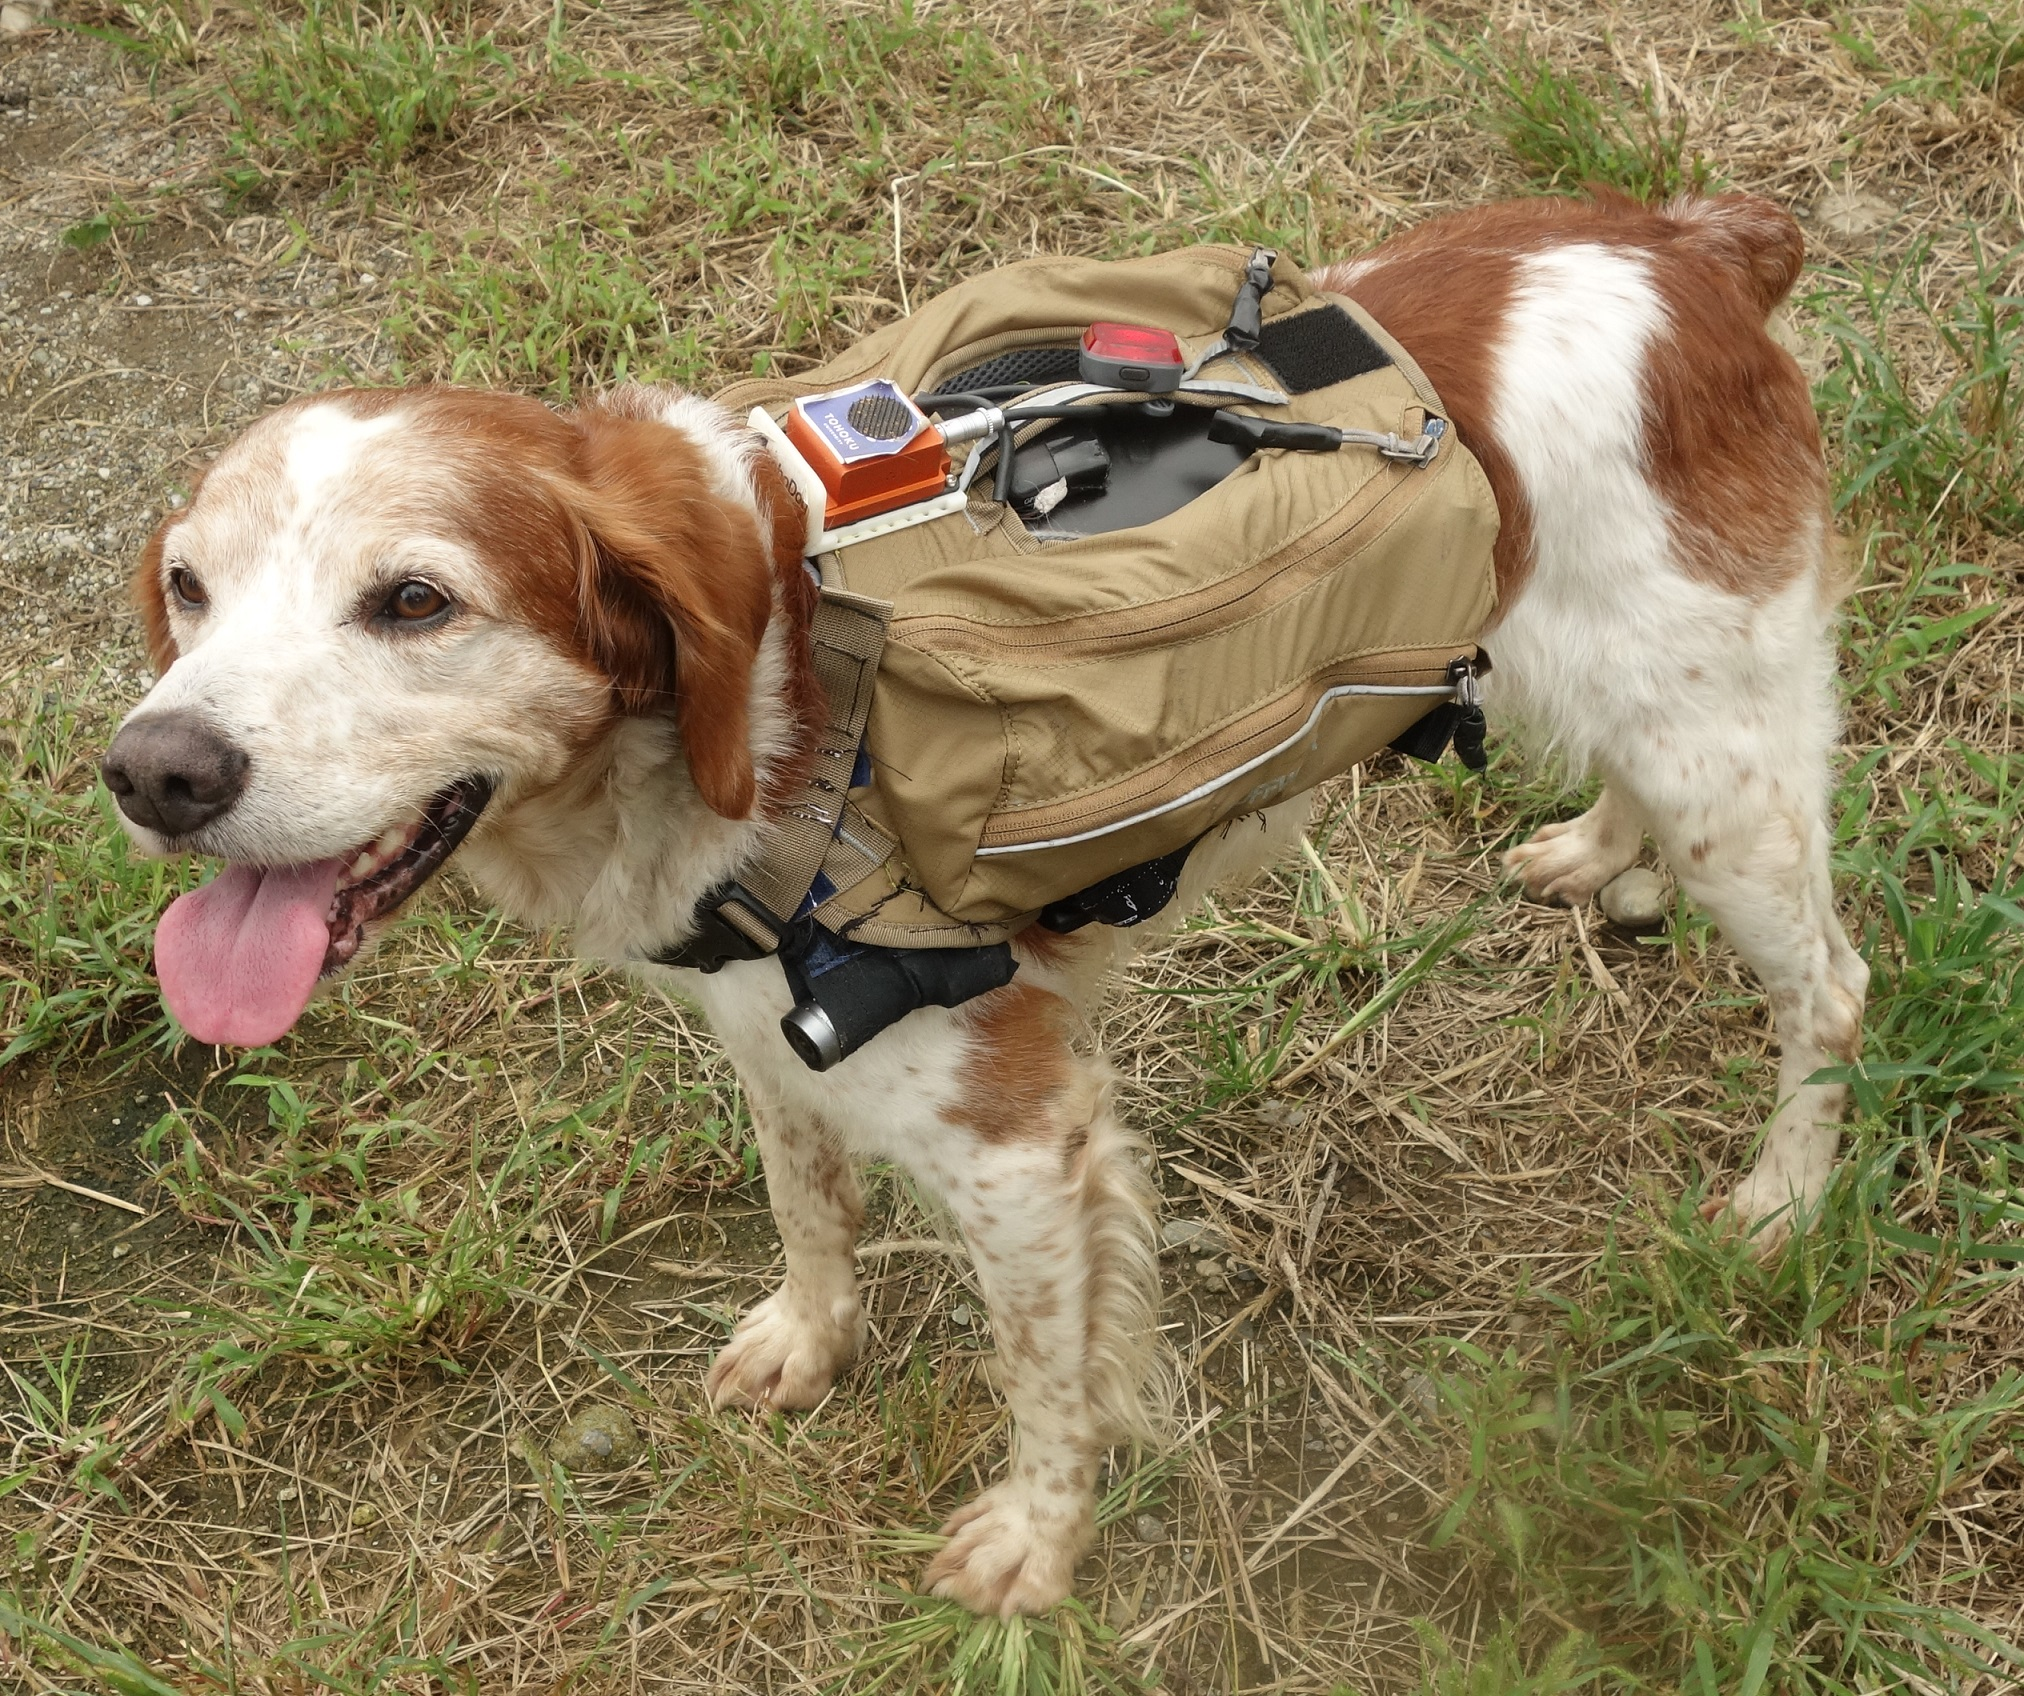
\includegraphics[width=6cm]{./Figures/cyberdog.eps}
  \caption{装着型計測・記録装置~\cite{dog01}より引用}
  \label{cyberdog}
 \end{center}
\end{figure}

また,Ehsanらによる犬の一人称視点動画からの犬行動予測の研究がある~\cite{whoretthedog}.これは,犬の行動をモデリングし,犬が次にどのような道をたどり行動するかを予測している.

%\section{問題点}
しかし,これらの研究は犬の行動のモデリングであり,犬の周辺環境の推定などは行っていない.また,入力は動画像のみであり,音声などのデータは利用していない.レスキュー犬の課題には,犬の周辺環境情報や動画像からだけでは判断できない情報の取得が含まれている.例えばレスキュー犬は要救助者を発見するとその場で待機し吠え続けるように訓練されている.このように,動画像データからだけではなく,音声データ,および慣性データ・GPSデータなどの情報を複合的に用いてレスキュー犬の状態を判断しなければならない.本研究は動画像と音声からなるマルチモーダルな情報を入力とした犬の行動の分類を目的としている. 

\section{画像認識}
\section{動画認識}
\subsection{Optical flow}
\subsubsection{FlowNet2.0}
\subsection{Two-stream}
\subsection{3D Convolution}
\section{音声分類}
\subsection{Sound Net}
\subsection{Audio-Visual Scene Analysis}
